\documentclass[12pt]{article}

% Packages
\usepackage[utf8]{inputenc}
\usepackage{amsmath, amssymb, amsthm}   % Math
\usepackage{graphicx}           % Images
% \usepackage{hyperref}           % Clickable links
\usepackage{geometry}           % Page margins
% \usepackage{cite}               % Citation formatting
\usepackage{algorithm}
\usepackage{algpseudocode}
\usepackage{listings}
\usepackage{color}

\definecolor{dkgreen}{rgb}{0,0.6,0}
\definecolor{gray}{rgb}{0.5,0.5,0.5}
\definecolor{mauve}{rgb}{0.58,0,0.82}

% BibLaTeX for references (requires biber)
\usepackage[
    backend=biber,
    style=numeric,
    sorting=nyt
]{biblatex}

\addbibresource{references.bib}  % Bib file

% Page setup
\geometry{margin=1in}

% Title
\title{Efficient entropy conversion using an entropy store}
\author{Calum Grant \\
OxFORD Asset Management \\
calum.grant@oxam.com}
\date{\today}

\newtheorem{lemma}{Lemma}
\newtheorem{corollary}{Corollary}
\newtheorem{definition}{Definition}
\newtheorem{theorem}{Theorem}

\lstset{
  language=C,        % choose the language
  basicstyle=\ttfamily\small, % font style and size
  keywordstyle=\color{blue},
  commentstyle=\color{gray},
  stringstyle=\color{orange},
  numbers=left,
  numberstyle=\tiny\color{gray},
  stepnumber=1,
  numbersep=5pt,
  showstringspaces=false,
  breaklines=true,
  frame=single,
  captionpos=b
}

\begin{document}

\maketitle

\begin{abstract}
    We present new algorithms for converting random integers between different forms using an \em entropy store \em to cache unused entropy. The method can generate exact random variables for any weighted integer distribution, and consume entropy from any such distribution, whilst losing almost no entropy in the process.  For example we can shuffle a deck of 52 cards using just $\approxeq 225.58102$ bits of entropy, yielding an entropy conversion efficiency of $\approxeq 0.99999992$ using a 32-bit entropy store, compared with classical "optimal" algorithms that only have $\approxeq 0.81$ efficiency.  The algorithm requires two 32-bit integer divmod operations per output, making it a bit slower than other methods.
\end{abstract}

\section{Introduction}

In this paper, we will study generating perfectly distributed integers from an entropy source. A typical example of this is using fair coin flips to roll a fair die or to perform a perfect shuffle of a deck of cards, but random numbers are ubiquitous in other areas such as security, AI, and simulations.

The general problem is one of \em entropy conversion \em, where entropy in one form needs to be converted to entropy in a different form using a function $f$ on a discrete random variable $X$ having Shannon entropy $H(X)$
\cite{shannon1948mathematical}.  
A fundamental result is that you cannot get more entropy out than you put in, or $H(X) \ge H(f(X))$. \cite{cover1999elements} 
We will be mainly focussed on improving the \em efficiency \em of entropy conversion, defined as $\eta = \frac{H(f(X))}{H(X)}$.

Whilst this problem has been studied extensively, there are theoretical limits on efficiency because algorithms must always fetch entropy in units, and any excess entropy is simply lost. An optimal algorithm must fetch up to 2 extra bits of entropy per output.  \cite{cover1999elements, Knuth1976TheCO}

To mitigate these entropy losses, it is possible to generate random integers in batches. The major drawback with batching schemes is that they do not scale very well and have limits on their capacity and efficiency.

In this paper we will explore a fundamentally different approach, by allowing entropy conversion algorithms access to an \em entropy store \em (ES) in the form of a large uniformly distributed integer, and allow the algorithm to put back any unused entropy into the store. An entropy store allows us to make efficient decisions and recover almost all lost entropy.

The entropy efficiency depends only on the ratio of the size of the store to the size of the number generated, and a precise bound is calculated in Theorem \ref{thm:loss}. 

For example to roll a 6-sided die with a 32-bit entropy store (holding at least 31 bits of entropy) has an entropy efficiency of $>0.99999997$. To shuffle a deck of 52 cards with a 32-bit entropy store has an entropy efficiency $>0.99999992$. By increasing the size of the store, we can achieve entropy efficiency arbitrarily close to 1.


\subsection {Contribution}

We present new algorithms, called \em entropy store algorithms \em, that have lower setup costs and higher amortised entropy efficiency than classical algorithms. Table \ref{tab:entropy-store} summarises the algorithm, where $m$ is the number of bits in each integer, and $n$ is the size of the distribution. $\epsilon$ is defined in Theorem \ref{thm:loss} and graphed in Figure \ref{fig:uniform-losses}. These characteristics are essentially optimal since $m$ and $n$ are usually constant.  For uniform or Bernoulli distributions, $n=O(1)$. A weighted distribution covers other distribution types such as uniform, rational weights, dyadic and Bernoulli distributions.

\begin{table}[h!]
\centering
\begin{tabular}{|c|c|c|c|c|}
\hline
Input & Output & Entropy & Time & Space \\
\hline
Weighted & Weighted & $H(P)+\epsilon$ & Setup: $O(mn)$ & Weighted: $O(mn)$ \\
Exact & Exact & (amortised) & Per output: $O(m \log m)$  &  Uniform/Bernoulli: \\
Markov & Markov &  &   & $O(m)$  \\
\hline
\end{tabular}
\caption{Entropy store algorithm overview.}
    \label{tab:entropy-store}
\end{table}

No other algorithm has achieved this level of entropy efficiency in practice.

\subsection{Related work}

Entropy conversion is a well studied subject going back to at least 1951 when Von Neumann \cite{neumann51} proposed the first known algorithm for generating perfectly uniform integers (a "dice roll") from an unbiassed coin (a "coin flip") - just three years after Claude Shannon's seminal work from 1948 \cite{shannon1948mathematical}. Von Neumann's rejection sampling algorithm works by fetching the smallest power of 2 greater or equal to the number being generated. If the number is in range, return it, otherwise retry. This algorithm is elegant but not optimal in its entropy efficiency.

Knuth and Yao \cite{Knuth1976TheCO} devised an optimal algorithm, based on creating a binary decision tree based on the arithmetic coding of each output, and proved that no other binary decision tree could on average give fewer decisions.

The drawbacks with the original Knuth-Yao algorithm are the setup and space costs: the decision trees are explicitly constructed can get quite large. Lumbruso \cite{lumbroso2013optimal} devised an optimal dice rolling algorithm, that is no more efficient than Knuth-Yao, but requires no setup and is simple to implement. Bacher et al \cite{bacher2017} analyse the Von Neumann and Knuth-Yao algorithms from an entropy perspective, using Lumbruso's implementation, with a particular focus on generating unbiased permutations from unbiased coin flips. There are always up to 2 bits of entropy loss (or 'toll') for each uniform integer generated, depending on the number being generated. Only exact powers of 2 can be generated without entropy loss.

Lemire \cite{lemire2019fast} compares different practical uniform generators, and describes a uniform generator that is efficient from a CPU perspective, but are very inefficient from an entropy perspective, by using fewer CPU division operations. Lemire's argument is that often the entropy comes from a pseudorandom source that can be quickly generated.

Various methods have been explored for generating arbitrary intervals.
The Knuth-Yao algorithm can be used to generate arbitrary distributions from binary entropy, but the tree may need to be truncated unless the distribution is dyadic.

The alias method devised by Walker \cite{walker1977efficient} and improved by Vose \cite{vose91} maps a uniform integer to an arbitrary distribution, and is therefore less entropy efficient because the output distribution generally contains less entropy than the uniform input distribution.

Han and Hoshi \cite{han97} devised an optimal interval algorithm to convert biased or unbiased coin-flips to an arbitrary distribution, with an overhead of up to 3 bits of entropy per output.  The algorithm works by dividing the $[0,1)$ real interval according to the output distribution, and stops at bit n when the fetched binary number falls entirely within the output interval in the nth bit. Han and Hoshi show that this algorithm has an asymptotically optimal entropy consumption. 
Wanatabe \cite{wanatabe20} analyses this algorithm using an information spectrum, and Oohama \cite{oohama11, oohama2020performance} analyses the performance this algorithm.

Saad et al \cite{saad2020fldr} introduce Fast Loaded Dice Roller (FLDR) algorithm and Draper and Saad \cite{draper2025efficient} the Amplified Loaded Dice Roller (ALDR) algorithms to generate more efficient discrete distribution generating trees (DDG). They observe that DDG-based algorithms like Knuth-Yao can be very large and slow, so propose a table-based approach with optimizations, which creates a faster random distribution generator within 2 bits per sample of the output entropy for ALDR, and 6 bits per output for FLDR.

\em Entropy extraction\em studies how to convert the entropy \em from \em a variety of different distributions. When the input distribution is unknown, Von Neumann \cite{neumann51} gives an algorithm to extract unbiased entropy from a biassed coin, which is again elegant but suboptimal in its entropy efficiency. Peres \cite{peres1992iterating} devised a way to recursively use the previously-discarded outputs to provide an algorithm with perfect amortised entropy efficiency, and the method was generalised by Pae \cite{pae15} to extract entropy from arbitrary but identically distributed unknown distributions ("weighted M-dice") with perfect amortised efficiency. Interestingly, it appears to be easier to extract entropy than to generate it.

Universal hashing can be used to turn unknown distributions into fair bits. Vembu et al \cite{vembu95} analyse the maximum rate at which entropy can be extracted. Goldreich's Leftover hash lemma \cite{goldreich2004foundations} calculates the length of possible output. Trevisan \cite{trevisan2001extractors} implements a universal hash extractor for unknown distributions with a known entropy. 

A common proposal to reach asymptotic efficiency for random number generation is to use batching to generate multiple outputs at the same time. \cite{bacher2017,han97,devroye86,Knuth1976TheCO,lumbroso2013optimal} Batching spreads the entropy loss over the batch size. However batching schemes suffer from increased size and complexity, and are less flexible because you must plan beforehand which numbers to generate. The fundamental limit to batching is that they do not scale well because they require arbitrary output precision or data structure sizes.






\section{Algorithms for entropy conversion}

In this section we'll start with some basic operations (Algorithm \ref{alg:combine}-\ref{alg:resample}), then use these to create an efficient generator for uniform integers (Algorithm \ref{alg:generate-uniform}) using an entropy store.

We'll then build on Algorithm \ref{alg:generate-uniform} to create a generator for an arbitrary weighted distribution (Algorithm \ref{alg:generate-distribution}), extract entropy from a weighted distribution (Algorithm \ref{alg:combine-distribution}), from which we can build a general entropy converter. All of these algorithms are designed to have a 1 or near-1 entropy efficiency, and proofs of correctness and efficiency are contained throughout this section.

We'll use uppercase letters $X$, $Y$ and $Z$ for discrete random variables, and write $H(X)$ for the Shannon entropy of this variable. Write $X \sim Uniform\{0..n-1\}$ to mean that $X$ is distributed with a uniform distribution, or $X \sim Uniform\{n\}$ for short, because all distributions will be 0-based. $H(Uniform\{n\}) = \log_2n$. The interval $[a,b)$ means all integers in the range $a...b-1$. Write $\mathbb{P}$ for probability, $\mathbb{E}$ for expected value, and $f$ as a function on random variables.


\subsection{Fundamental operations}

At the basis of the ES is the ability to extract entropy from a uniform distribution, and to combine entropy with a uniform distribution in an entropy-preserving way. 

The function $f_{combine}$, in Definition \ref{def:combine}, divides the range $[0,nm)$ into $n$ subranges of $[0,m)$ as follows:

\[
\overbrace{
    \underbrace{
        \underbrace{a_0 ... a_{m-1}}_{m}
        \underbrace{a_m ... a_{2m-1}}_{m}
        ...
        \underbrace{a_{n(m-1)}...a_{nm-1}}_{m} 
        }_{n}}
        ^{nm}
\]

\begin{definition}
    $f_{combine}: [0,n)\times [0,m) \rightarrow [0,nm)$ is defined as $f_{combine}(X,Y) = mX+Y$.
    \label{def:combine}
\end{definition}

$f_{combine}$ sets up a 1-1 correspondence, a bijection, between a uniform distribution $Uniform\{nm\}$ and a pair of independent uniform distributions $Uniform\{n\}$ and $Uniform\{m\}$. This will allow us to split and combine entropy in an entropy-preserving way. Similar constructs can be found for example in \cite{gentle2003xx} XX. 

\begin{lemma}
    The inverse of $f_{combine}$, $f^{-1}_{combine}(Z) = (\lfloor \frac{Z}{m} \rfloor, Z \mod m)$.
\end{lemma}

\begin{proof}
    $f_{combine}(f^{-1}_{combine}(Z)) = f_{combine}(\lfloor \frac{Z}{m}\rfloor, Z \text{ mod } m) = m(\lfloor \frac{Z}{m}m \rfloor) + (Z \mod m) = Z$. $f^{-1}_{combine}(f_{combine}(X,Y)) = f^{-1}_{combine}(mX+Y) = (\lfloor\frac{mX+Y}{m}\rfloor, (mX+Y)\mod m) = (X,Y)$.
\end{proof}

\begin{corollary}
    $f_{combine}$ is a bijection.
\end{corollary}

\begin{lemma}
    If $X \sim Uniform\{n\}$ and $Y \sim Uniform\{m\}$ are independent, then 
    $f_{combine}(X,Y) \sim Uniform \{nm\}$.
\end{lemma}

\begin{proof}
    Let $Z = mX+Y$, so $Z \in [0,nm)$. $\mathbb{P}(X=x,Y=y) = \mathbb{P}(X=x)\mathbb{P}(Y=y) = \frac{1}{n}\frac{1}{m} = \frac{1}{nm}$. Since $f_{combine}$ is a bijection then it means that all $z$ values occur with $\mathbb{P}(Z=z) = \frac{1}{nm}$, so $Z \sim Uniform\{nm\}$.
    
\end{proof}

\begin{lemma}
    If $Z \sim Uniform \{nm\}$, and $f^{-1}_{combine}(Z) = (X,Y)$, then $X \sim Uniform\{n\}$ and $Y \sim Uniform\{m\}$. $X$ and $Y$ are independent.
\end{lemma}

\begin{proof}
    Since $f_{combine}$ is a bijection, for all all values $\mathbb{P}(X=x,Y=y) = \frac{1}{nm}$.

    $\mathbb{P}(X=x) = \sum_{y}\mathbb{P}(X=x,Y=y) = m\frac{1}{nm} = \frac{1}{n}$. $\mathbb{P}(Y=y) = \sum_{x}\mathbb{P}(X=x,Y=y) = n\frac{1}{nm} = \frac{1}{m}$. This proves that $X\sim Uniform\{n\}$ and $Y\sim Uniform\{m\}$.

    $\mathbb{P}(X=x,Y=y) = \frac{1}{nm} = \mathbb{P}(X=x)\mathbb{P}(Y=y)$, so $X$ and $Y$ are independent.
\end{proof}

Algorithm \ref{alg:combine} is an implementation of $f_{combine}$, and Algorithm \ref{alg:divide} is an implementation of $f^{-1}_{combine}$. Algorithm \ref{alg:combine} will be used when \em returning \em entropy to the entropy store, and Algorithm \ref{alg:divide} can be used to extract entropy from the entropy store.

\begin{algorithm}
\caption{Combining uniformly distributed integers}
\label{alg:combine}
\begin{algorithmic}[1]
    \Require $n$, $m$, $U_n$, $U_m$ are integers
    \Require $n>0$, $m>0$
    \Require $U_n$ is uniformly distributed over $[0,n)$
    \Require $U_m$ is uniformly distributed over $[0,m)$
    \Require $U_n$ and $U_m$ are independently distributed
    \Ensure $nm$ is $n * m$
    \Ensure $U_{nm}$ is uniformly distributed over $[0,nm)$
\Procedure{combine}{$U_n, n, U_m, m$} 
  \State $U_{nm} \gets U_n * m + U_m$
  \State $nm \gets n * m$
  \State \Return $U_{nm}, nm$
\EndProcedure
\end{algorithmic}
\end{algorithm}

\begin{algorithm}
\caption{Division of uniformly distributed integers}
\label{alg:divide}
\begin{algorithmic}[1]
    \Require $nm$, $n$, $U_{nm}$ are integers
    \Require $nm>0$, $m>0$
    \Require $nm$ is divisible by $n$
    \Require $U_{mn}$ is uniformly distributed over $[0,nm)$
    \Ensure $n * m = nm$
    \Ensure $U_{n}$ is uniformly distributed over $[0,n)$
    \Ensure $U_{m}$ is uniformly distributed over $[0,m)$
    \Ensure $U_n$ and $U_m$ are independent
\Procedure{divide}{$U_{nm}, mn, n$} 
  \State $U_m \gets U_{nm} \operatorname{div} n$
  \State $U_{n} \gets U_{nm} \mod n$
  \State $m \gets nm / n$
  \State \Return $U_m, m, U_n$
\EndProcedure
\end{algorithmic}
\end{algorithm}


The function $f_{sample}$, in Definition \ref{def:sample}, divides the range $[0,n)$ into two parts:

\[
\overbrace{
    \underbrace{
        \underbrace{a_0 \text{   } ... \text{   } a_{m-1}}_{m}
        \underbrace{a_m \text{   } ... \text{   } a_{n-1}}_{n-m}}
    }_{Bernoulli\{\frac{m}{n}\}}^{n}
\]

\begin{definition}
$f_{sample}: [0,n) \rightarrow \{0,1\} \times [0,\max(n,n-m))$ is defined as $f_{sample}(Z) = (Z<m, m(Z\ge m) + Z).$. (Assume that the operators $<$ and $\ge$ evaluate to $0$ or $1$.)
\label{def:sample}
\end{definition}

When $Z$ is uniformly distributed, then its outputs will be Bernoulli distributed and uniformly distributed. $f_{sample}$ is reversible, meaning it has an inverse that can be used to combine a Bernoulli distribution with a uniform distribution to create a larger uniform distribution (whose entropy equals the sum of the original distributions).

proofs here...

Algorithm \ref{alg:downsample} implements $f_{sample}$ and Algorithm \ref{alg:upsample} implements $F^{-1}_{sample}$. Algorithm \ref{alg:downsample} can be used to resize a uniform distribution or to generate a Bernoulli variable. Algorithm \ref{alg:upsample} ....


\begin{algorithm}
\caption{Resampling uniformly distributed integers}
\label{alg:downsample}
\begin{algorithmic}[1]
    \Require $U_{n}$, $m$ and $n$ are integers 
    \Require $0 \le m \le n$
    \Require $U_{n}$ is uniformly distributed over $[0,n)$
\Ensure $U_{x}$ is uniformly distributed over $[0,x)$
\Ensure $x = m$ or $x=n-m$
\Ensure $B$ is a Boolean value Bernoulli distributed with $p=\frac{m}{n}$
\Ensure $U_x$ and $B$ are independent
\Procedure{resample}{$U_n, n, m$} 
  \If{$U_n < n$}
    \State $B \gets True$  
    \State $x \gets m$
    \State $U_x \gets U_n$
  \Else
    \State $B \gets False$  
    \State $x \gets n-m$
    \State $U_x \gets U_n-m$
  \EndIf
  \State \Return $U_x, x, B$
\EndProcedure
\end{algorithmic}
\end{algorithm}

\begin{algorithm}
\caption{Resampling uniformly distributed integers}
\label{alg:upsample}
\begin{algorithmic}[1]
    \Require $U_{x}$ is uniformly distributed over $[0,x)$
    \Require $x = m$ or $x=n-m$
    \Require $B$ is a Boolean value Bernoulli distributed with $p=\frac{m}{n}$
    \Require $U_{n}$, $m$ and $n$ are integers 
    \Ensure $U_x$ and $B$ are independent
    \Ensure $U_{n}$ is uniformly distributed over $[0,n)$
\Procedure{downsample}{$xx$} 
    \State $123$
\EndProcedure
\end{algorithmic}
\end{algorithm}


Algorithm \ref{alg:downsample} is the basis for von Neumann's rejection sampling algorithm, and Lumbrusco's fast dice roller algorithm. However these algorithms throw away some of the outputs, resulting in entropy loss.

\subsection{Generating uniform integers}

Algorithm \ref{alg:generate-uniform} reads binary entropy from a $fetch()$ function, and outputs a uniform integer in the range $[0,n)$. The algorithm makes use of an \em entropy store \em $U_s$ which is carried over in between function calls. Initially the entropy store is empty (containing $0$ entropy) with $U_s = 0$ and $s=1$.

The overall strategy of Algorithm \ref{alg:generate-uniform} is to use $resample$ (Algorithm \ref{alg:resample}) to ensure that $s$ is a multiple of $n$, then use the $divide$ algorithm (Algorithm \ref{alg:divide}) to divide $U_s$ into $U_n$. $U_n$ is returned as the result, and $U_s$ which is stored for the next invocation. The calculation is structured so that when $s$ is large, the entropy lost by $resample$ is very small.

The $resample$ on line 6 resizes $s$ to a multiple of $n$. It is overwhelmingly likely that $b$ is false because $n$ is much smaller than $s$, so we can then proceed to line 8 where we divide $U_s$ into $U_n$ and the new $U_s$. On line 9, return $U_n$ as the result and $U_s$ and $s$ as the input to the next invocation.

An C implemetation of Algorithm \ref{alg:generate-uniform} is given in Appendix \ref{adx:source}.

\begin{algorithm}
\caption{Generating uniformly distributed integers}
\label{alg:generate-uniform}
\begin{algorithmic}[1]
\Require Integers $0 < n\le N$
\Require $fetch()$ returns Bernoulli entropy with $p=0.5$
\Require $U_s$ is uniformly distributed over $[0,s)$
\Ensure $U_n$ is uniformly distributed over $[0,n)$
\Ensure $U_s$ is uniformly distributed over $[0,s)$
\Procedure{generate\_uniform}{$U_s, s, n, N$} 
  \While {True}
    \While {$s < N$}
        \State $U_s, s \gets combine(U_s, s, fetch(), 2)$
    \EndWhile
    \State $U_s, s, b \gets resample(U_s, s, s \mod n)$ 
    \If{$ \neg b$}
        \State $U_n, U_s, s \gets divide(U_s, s, n)$
        \State \Return $U_s, s, U_n$
    \EndIf
  \EndWhile
\EndProcedure
\end{algorithmic}
\end{algorithm}

\begin{lemma}
    In Algorithm \ref{alg:generate-uniform}, 
$U_n$ is uniformly distributed over $[0,n)$ and 
$U_s$ is uniformly distributed over $[0,s)$.
\end{lemma}

\begin{proof}
The values $U_n$, $n$, $U_s$ and $s$ have been generated by Algorithms \ref{alg:combine}, \ref{alg:divide} and \ref{alg:resample}. By Lemmas \ref{lem:combine}, \ref{lem:divide} and \ref{lem:resample}, $U_n$ and $U_s$ are uniformly distributed.
\end{proof}

Algorithm \ref{alg:generate-uniform} terminates with probability 1.

\begin{lemma}
    \label{lem:shannon-inequality}

For $p,q \in \mathbb{R}$, where $0 \le p\le q \le 0.5$, 

\begin{equation}
-p\log_2 p - (1-p)\log_2(1-p) \le -q\log_2 q - (1-q)\log_2(1-q)
\end{equation}
\end{lemma}

\begin{proof}
    Let
    \begin{align}
        g(p) & = -p\log_2 p - (1-p)\log_2(1-p) \\
        \implies g'(p) & = \log_2\frac{1-p}{p} = \log_2(\frac{1}{p}-1) \ge \log_21 = 0 
    \end{align}
Since the derivative of $g>0$ it means that $g$ is monotonic.
\end{proof}

\begin{definition}
    Let $\epsilon = \epsilon(p)$ be the expected entropy loss function of Algorithm \ref{alg:generate-uniform}, where $p=\frac{n-1}{N}$.
\end{definition}

\begin{theorem}
    \label{thm:loss}
If $p = \frac{n-1}{N} < 0.5$, then

\begin{equation}
0 \le \epsilon(p) \le -\frac{p}{1-p}\log_2p - \log_2(1-p)
\end{equation}

\end{theorem}

\begin{proof}
For each iteration $i$ of Algorithm \ref{alg:generate-uniform}, let $p_i = \frac{s_i \mod n}{s_i}$. But $(s_i \mod n) \le n-1$ and $s_i \ge N$, so $\frac{s_i \mod n}{s_i} \le \frac{n-1}{N}$, so $p_i \le p$. On each iteration, the entropy lost is equal to the entropy in the variable $b_i \sim Bernoulli\{p_i\}$, which is given by the entropy equation for a Bernoulli distribution \cite{cover1999elements}:

\begin{equation}
H(b_i) = -p_i\log_2p_i - (1-p_i)\log_2(1-p_i)
\end{equation}

Therefore, 

\begin{equation}
0 \le H(b_i) \le -p\log_2p - (1-p)\log_2(1-p) 
\end{equation}


by Lemma \ref{lem:shannon-inequality}. The expected number of iterations $N$ is given by

\begin{align}
& N = 1 + p_iN \le 1 + pN \\
\implies & N-pN \le 1 \\
\implies & N(1-p) \le 1 \\
\implies & N \le \frac{1}{1-p}
\end{align}

The total entropy lost by the algorithm is given by the number of iterations of the algorithm multiplied by the entropy lost in each iteration.

\begin{align}
0 \le NH(b_i) \le & \frac{1}{1-p}(-p\log_2p - (1-p)\log_2(1-p) ) \\
= & -\frac{p}{1-p}\log_2p - \log_2(1-p)
\end{align}

We can also end up in the situation where $(s \mod n) = 0$ already, in which the \em resample \em step always succeeds with no entropy loss, so $\epsilon=0$.
\end{proof}

The actual entropy loss incurred by Algorithm \ref{alg:generate-uniform} depends on whatever values are found in $U_s$ and $s$, so we can only give an upper bound.

\begin{corollary}
The entropy efficiency $\eta$ of Algorithm \ref{alg:generate-uniform} is bounded by

\begin{equation}
\frac{\log_2n}{\log_2n + \epsilon(\frac{n-1}{N})} \le \eta \le 1
\label{eq:generate-uniform-efficiency}
\end{equation}
\end{corollary}

\begin{proof}
\begin{align}
    \eta & = \frac{H_{out}}{H_{in}} \\
         & = \frac{H_{out}}{H_{out}+\epsilon} \\
         & = \frac{\log_2n}{\log_2n + \epsilon(\frac{n-1}{N})}
\end{align}
Therefore 
\begin{equation}
\frac{\log_2n}{\log_2n + \epsilon(\frac{n-1}{N})} \le \eta \le 1
\end{equation}
from Theorem \ref{thm:loss}.
\end{proof}

To illustrate Equation \ref{eq:generate-uniform-efficiency}, if $N=2^{31}$ and $n=6$, then $\eta \ge 0.99999997$. This means that even with a modest entropy buffer, we can get very good entropy efficiency.

\begin{corollary}
The entropy efficiency $\eta$ of Algorithm \ref{alg:generate-uniform} is arbitrarily close to 1.
\end{corollary}

\begin{proof}
$\epsilon(\frac{n-1}{N}) \rightarrow 0$ as $N \rightarrow \infty$, using L'H\^opital's Rule. Therefore $\eta \rightarrow 1$ as $N \rightarrow \infty$.
\end{proof}



\subsection{Generating Bernoulli distributions}




\subsection{Generating weighted integer distributions}

Algorithm \ref{alg:generate-distribution} shows how we can generate an arbitrary  distribution of $k$ outcomes where each outcome has integer weight $\{w_0, w_1, ..., w_{k-1}\}$, normalised to a discrete distribution with probabilities $\{\frac{w_0}{n}, \frac{w_1}{n}, ..., \frac{w_{k-1}}{n}\}$ where $n=\sum_i w_i$ is the total weight.

The algorithm works by constructing a surjective mapping from the $n$ outcomes of a uniform distribution to the $k$ outputs of the weighted distribution. This uses a simple lookup table of size $n$, constructed using Algorithm \ref{alg:generate-lookup-tables}. If $n$ is very large we could implement the mapping as a binary search on $offset$ instead. To generate an output, call $generate\_uniform$ to generate a integer in the range $[0,n)$, and use the number in the $output$ lookup table as the result. 

We would expect this process to lose entropy because in general the output distribution contains less entropy than the input distribution. The new idea is that we can recover all of the entropy from this process. By splitting up $[0,n)$ into chunks of size $w_i$, each value in $[0,n)$ is contained in a uniform distribution $Uniform\{w_i\}$.

\[
\overbrace{
    \underbrace{
        \underbrace{a_0 ... a_{w_0-1}}_{w_0}
          \underbrace{a_{w_0} ... a_{w_0+w_1-1}}_{w_1}
          ...
          \underbrace{
             a_{n-w_{k-1}} ... 
             a_{n-1}
         }_{w_{k-1}}
    }_{Weighted\{w_0, ..., w_{k-1}\}}
}^{n}
\]

The chunk contains $\log_2w_i$ entropy. We can use $combine$ to return this entropy back to the entropy store. Lemma \ref{lem:distribution-conservation} shows us that when we account for this extra entropy then no entropy is lost.



\begin{definition}
    Let $f_{distribute}: X \rightarrow Y, Z$ be the function that maps random variable $X \sim Uniform\{n\}$ to independent random variables $Y$ and $Z \sim Uniform\{w_i\}$.

    \begin{align}
    Y &= max(j : \sum_{i<j}w_i<X) \\
    Z &= X - \sum_{i<Y}w_i
    \end{align}

\end{definition}

Note that $f_{distribute}$ is a generalisation of XX $f_{combine}$ and $f_{sample}$ XX we didn't define $f_{sample}$.

\begin{lemma}
    \label{lem:distribution-conservation}
    $f_{distribute}$ does not lose entropy
\end{lemma}

\begin{proof}
    \begin{align}
    \mathbb{E}(H(X)) & = \log_2 n \\
    \mathbb{E}(H(Y) + H(Z)) &=  \mathbb{E}(H(Y)) + \mathbb{E}(H(Z)) \\
               & = - \sum_i p_i \log_2p_i + \sum_i p_iH(Y|X=i) \\
               & = - \sum_i \frac{w_i}{n} \log_2 \frac{w_i}{n} + \sum_i \frac{w_i}{n}\log_2 w_i \\
               & = - \sum_i \frac{w_i}{n}(\log_2 w_i - \log_2 n) + \sum_i \frac{w_i}{n}\log_2 w_i \\
               & = - \sum_i \frac{w_i}{n}\log_2 w_i + \sum_i \frac{w_i}{n} \log_2 n + \sum_i \frac{w_i}{n}\log_2 w_i \\
               & = \sum_i \frac{w_i}{n} \log_2 n \\
               & = \frac{\log_2 n}{n} \sum_i w_i \\
               & = \frac{\log_2 n}{n} n \\
               & = \log_2 n
    \end{align}
\end{proof}

\begin{algorithm}
\caption{Constructing lookup tables for a weighted random variable}
\label{alg:generate-lookup-tables}
\begin{algorithmic}[1]
\Require $weights$ is a list of integers $\ge0$
\Procedure{make\_distribution}{$weights$} 
  \State $outputs \gets []$
  \State $offsets \gets []$
  \For {$w_i \in weights$}
    \State $offsets \gets offsets + [|outputs|]$
    \State $outputs \gets outputs + [i] * w_i$
  \EndFor
  \State \Return $outputs, offsets$
\EndProcedure
\end{algorithmic}
\end{algorithm}


\begin{algorithm}
\caption{Generating a weighted random variable}
\label{alg:generate-distribution}
\begin{algorithmic}[1]
\Require $U_s$, $s$, $N$ are integers
\Require $weights$ is an array of integers $w_i \ge 0$
\Require $offset$ generated by $make\_distribution$ 
\Require $outputs$ generated by $make\_distribution$
\Require $U_s$ is uniformly distributed over $[0,s)$
\Require $N >> |outputs|$
\Ensure $U_s$ is uniformly distributed over $[0,s)$
\Procedure{generate\_distribution}{$U_s, s, N, weights, outputs, offsets$} 
    \State $n \gets |outputs|$
    \State $U_s, s, U_n \gets generate\_uniform(U_s, s, N, n)$
    \State $U_s, s = combine(U_s, s, U_n - offsets[U_n], weights[outputs[U_n]])$
    \State \Return $U_s, s, outputs[U_n]$
\EndProcedure
\end{algorithmic}
\end{algorithm}


\begin{lemma}
The inverse of $f_{distribute}$ is given by

    \begin{equation}
    f^{-1}_{distribute}(Y,Z) = \sum_{i<Y}w_i + Z
    \end{equation}
\end{lemma}

\begin{proof}
    Show that $f^{-1}f= I$

\end{proof}

\subsection {Extracting entropy from weighted integer distributions}

Algorithm \ref{alg:combine-distribution} performs the inverse of Algorithm \ref{alg:generate-distribution}. It reconstructs a uniform distribution $X$ of size $n$ from the weighted random variable $Y$, and combines it with a uniform distribution $Z$ of size $w_i$. This allows the entropy store to absorb the entropy from $i$.

Note that when performing the inverse of Algorithm \ref{alg:generate-distribution}, we don't need to supply it the *same* random variable $U_x$ that was originally used, and we can just get one from our entropy store.

We'll ignore potential integer overflows of $U_s$ and $s$.

\begin{algorithm}
\caption{Extracting entropy from a weighted random variable}
\label{alg:combine-distribution}
\begin{algorithmic}[1]
\Require $U_s$, $s$, $N$ are integers
\Require $weights$ is an array of integers $w_i \ge 0$
\Require $offset$ generated by $make\_distribution$ 
\Require $outputs$ generated by $make\_distribution$
\Require $U_s$ is uniformly distributed over $[0,s)$
\Require $N >> |outputs|$
\Ensure $U_s$ is uniformly distributed over $[0,s)$
\Procedure{combine\_distribution}{$U_s, s, N, weights, outputs, offsets, i$} 
    \State $U_s, s, U_x \gets generate\_uniform(U_s, s, N, weights[i])$
    \State $U_s, s \gets combine(U_s, s, U_x + offsets[i], |outputs|)$
    \State \Return $U_s, s$
\EndProcedure
\end{algorithmic}
\end{algorithm}



\begin{lemma}
    \label{lem:hloss_monotonic}
    $\epsilon(p)$ is monotonically increasing in the range $0 < p < 1$.
\end{lemma}

\begin{proof}The derivative of $\epsilon(p)$ is
    \begin{equation}
        \frac{-\log_2p}{(1-p)^2}
    \end{equation}
    which is positive in the range $0 < p < 1$.
\end{proof}

\begin{lemma}
The entropy loss of Algorithm \ref{alg:combine-distribution} is no more than than $\epsilon(\frac{n-1}{N})$
\end{lemma}

\begin{proof}
    The entropy-losing step in Algorithm \ref{alg:combine-distribution} is $generate\_uniform$ which loses $\epsilon(\frac{x-1}{N})$ bits. $x \le n$, so from Lemma \ref{lem:hloss_monotonic}, this means that $\epsilon(\frac{x-1}{N}) \le \epsilon(\frac{n-1}{N})$.
\end{proof}

To create a generic entropy converter between weighted distributions, we can use Algorithm \ref{alg:generate-distribution} to generate the output distribution, but replace the $fetch$ step in Algorithm \ref{alg:generate-uniform} with a call to $combine\_distribution$.





\section {Evaluation}

We have already shown that the entropy store (ES) algorithms are more efficient than optimal classical algorithms such as Knuth-Yao (KY) and the Interval Algorithm (IA), but it is still instructive to visualise this comparison.

Figure \ref{fig:uniform-losses} shows the calculated entropy loss for generating uniform integers, comparing ES methods with von Neumann (vN) and Knuth-Yao generators. These graphs show exact calculation unless stated otherwise. We can observe that for vN and KY, the entropy loss depends on the number being generated. KY loses up to 2 bits per output. ES is not dependent on the generated integer, but loses efficiency at high $n$ as it approaches its minimum store size $N$. We also show real world entropy loss, which depends on the previous size of the store, and it is within the worst case bound $\epsilon$. As expected, using a larger entropy buffer yields greater efficiency, but would be at the cost of a larger pre-fetch of entropy and slower divmod operations. \cite{Abel19a} compares the instruction latency on Intel CPUs, showing for example that on an Alder Lake-P CPU a 64-bit IDIV instruction takes 14-18 cycles compared with 10-15 cycles for 32-bit instructions.

\begin{figure}[ht]
\centering
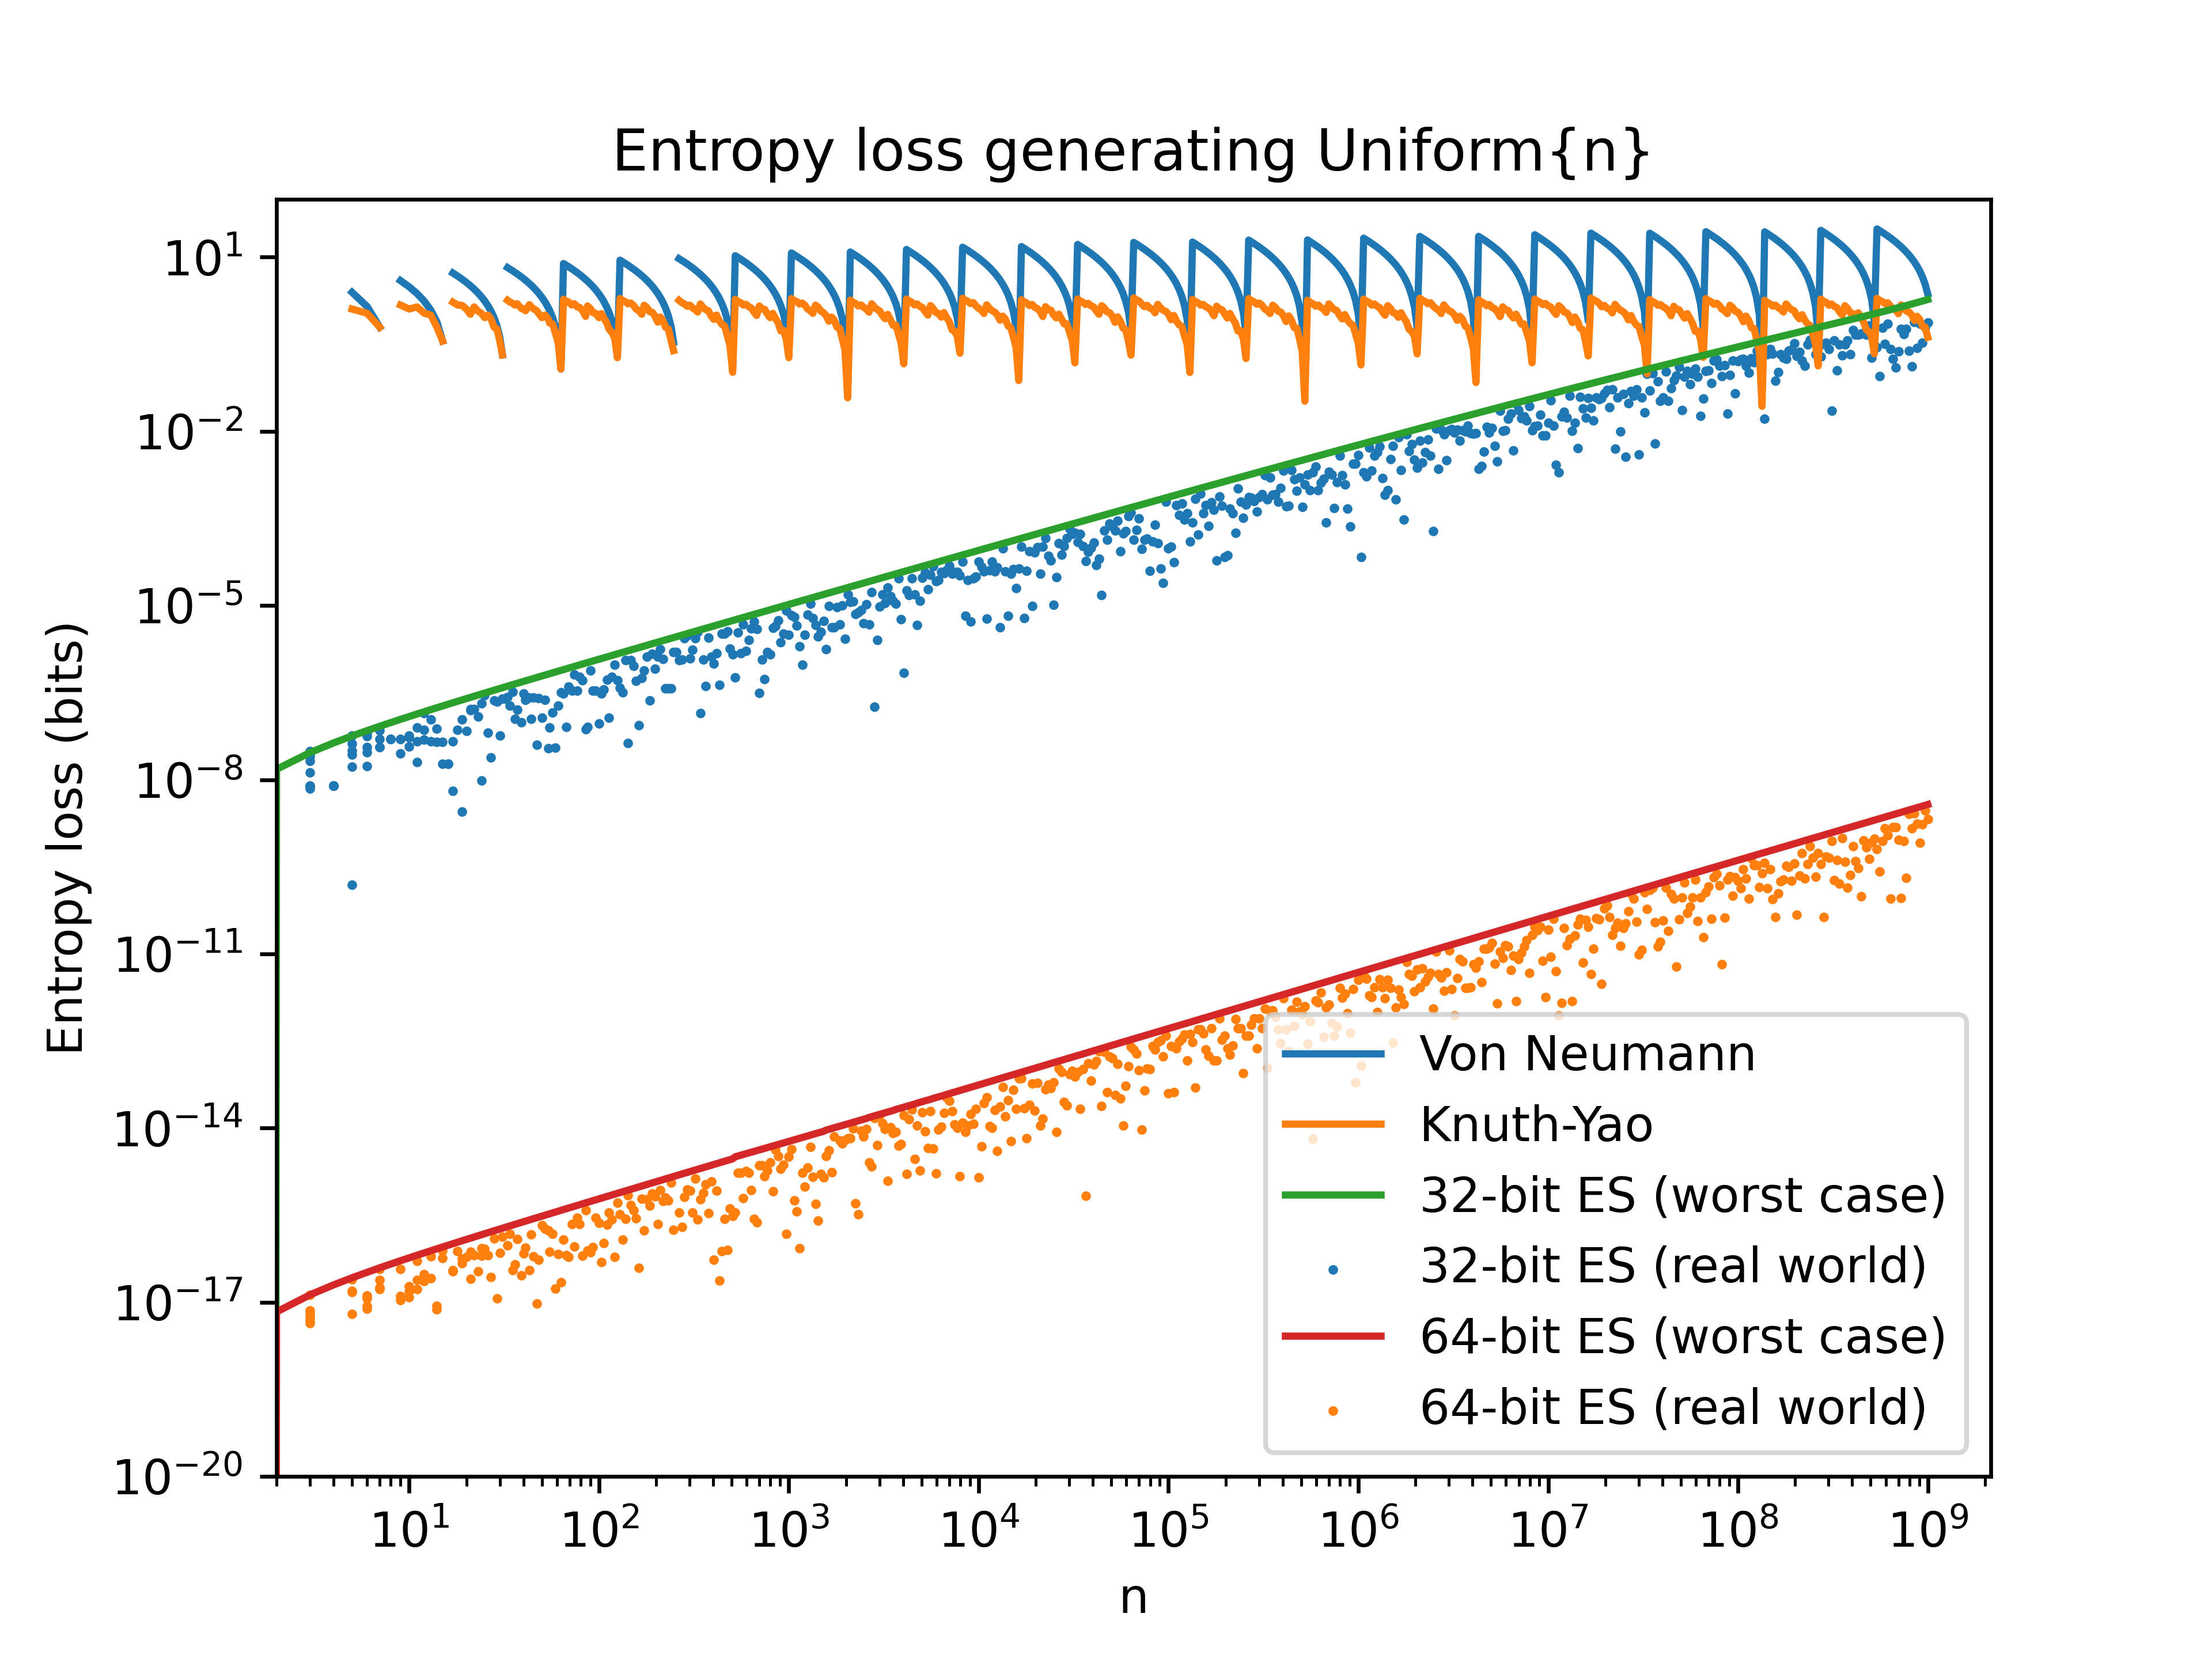
\includegraphics[width=0.8\textwidth]{uniform_losses.png}
\caption{Entropy losses for uniform integer generation.}
\label{fig:uniform-losses}
\end{figure}

Figure \ref{fig:shuffling-efficiency} shows the overall impact of entropy losses when applied to the shuffling a deck of $n$ cards using the Fisher-Yates algorithm \cite{fisher1953statistical, durstenfeld1964algorithm, knuth2014art}. This is a good demonstration of the entropy efficiency under a real-world workload. Calculations show that we can calculate that shuffling a deck of 52 cards can be done with an entropy loss of $\approxeq 1.7e-5$ bits, or an entropy efficiency of $\approxeq 0.99999992$.

\begin{figure}[ht]
\centering
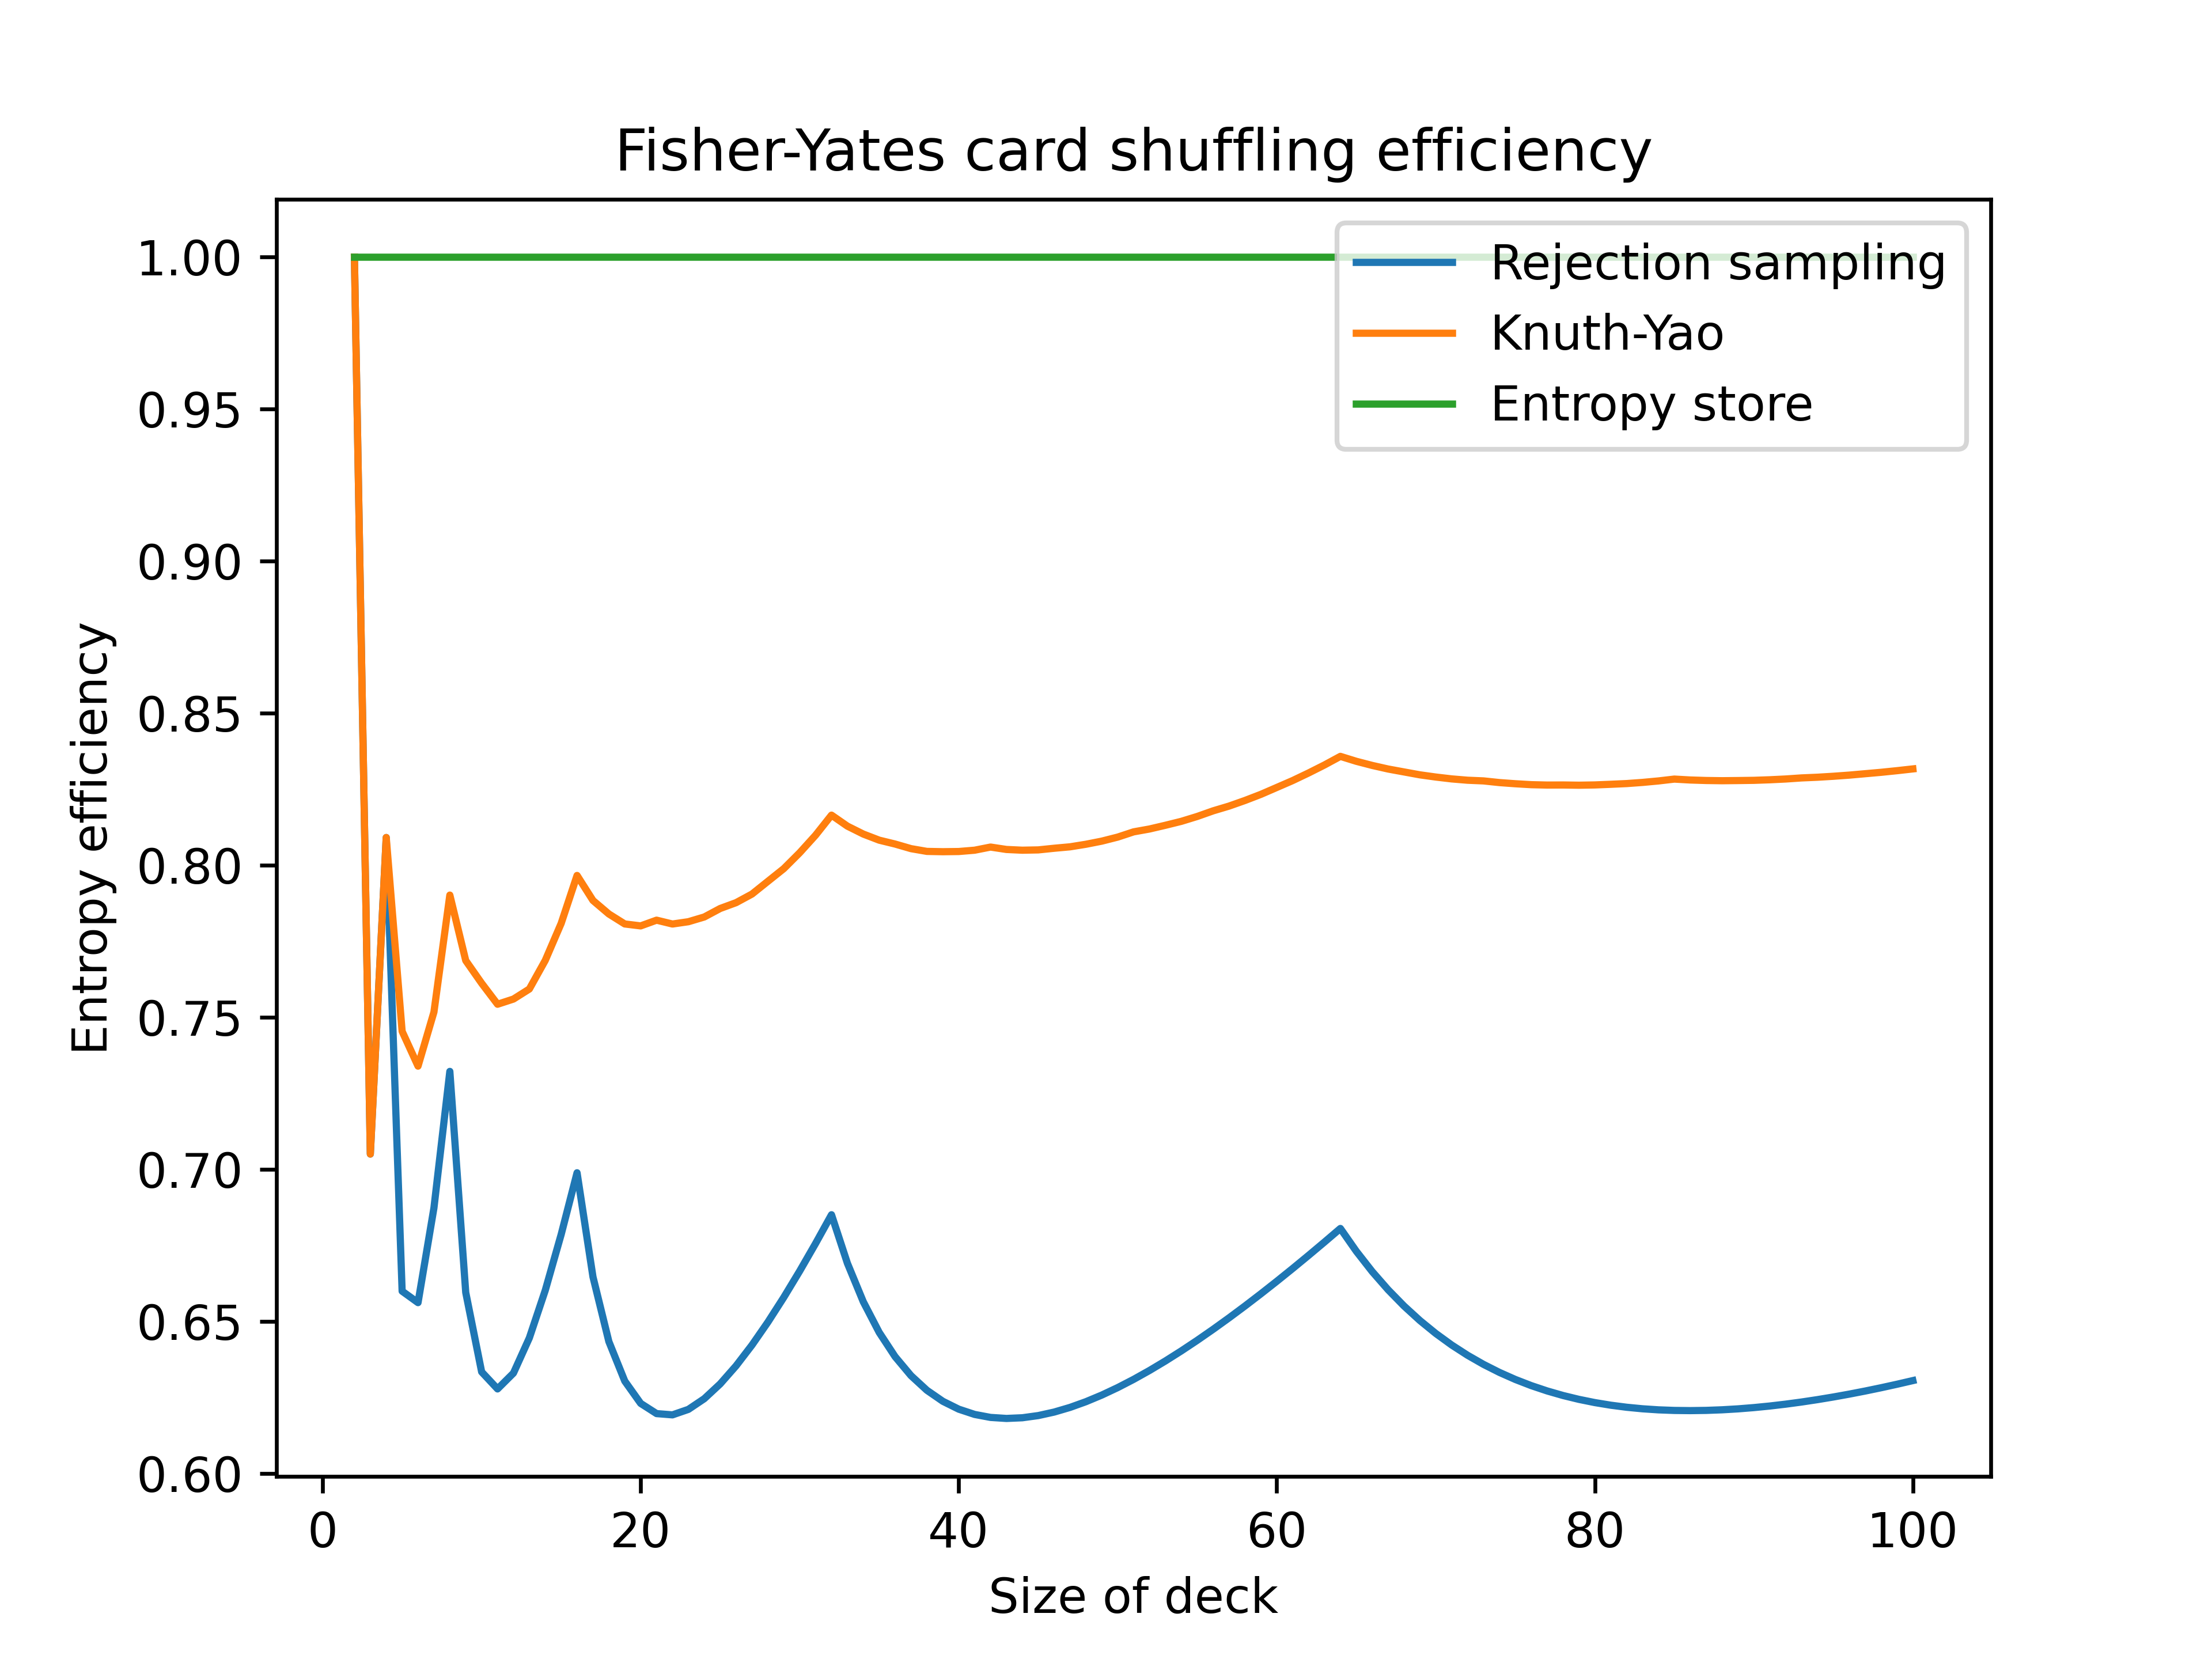
\includegraphics[width=0.8\textwidth]{shuffling_efficiency.png}
\caption{Entropy efficiency shuffling cards.}
\label{fig:shuffling-efficiency}
\end{figure}

When generating Bernoulli variables, we see in Figure \ref{fig:bernoulli-efficiency} that the entropy efficiency of the interval algorithm drops off significantly. IA must fetch between 1 and 2 bits per output on average. By contrast, ES algorithms to not necessarily fetch any bits to generate an output, as there may be enough entropy in the store already, so ES just shrinks the size of its store to generate an output. Figure \ref{fig:bernoulli-rate} shows that IA cannot increase its output rate as the entropy of the output distribution decreases below 1.

\begin{figure}[ht]
\centering
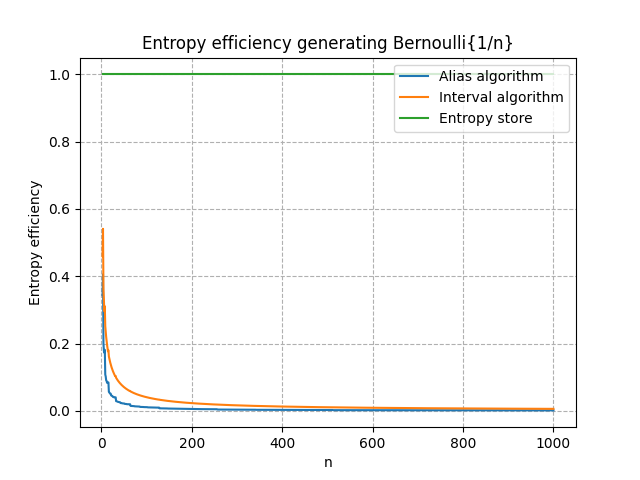
\includegraphics[width=0.8\textwidth]{bernoulli_efficiency.png}
\caption{Entropy efficiency generating Bernoulli distributions.}
\label{fig:bernoulli-efficiency}
\end{figure}

\begin{figure}[ht]
\centering
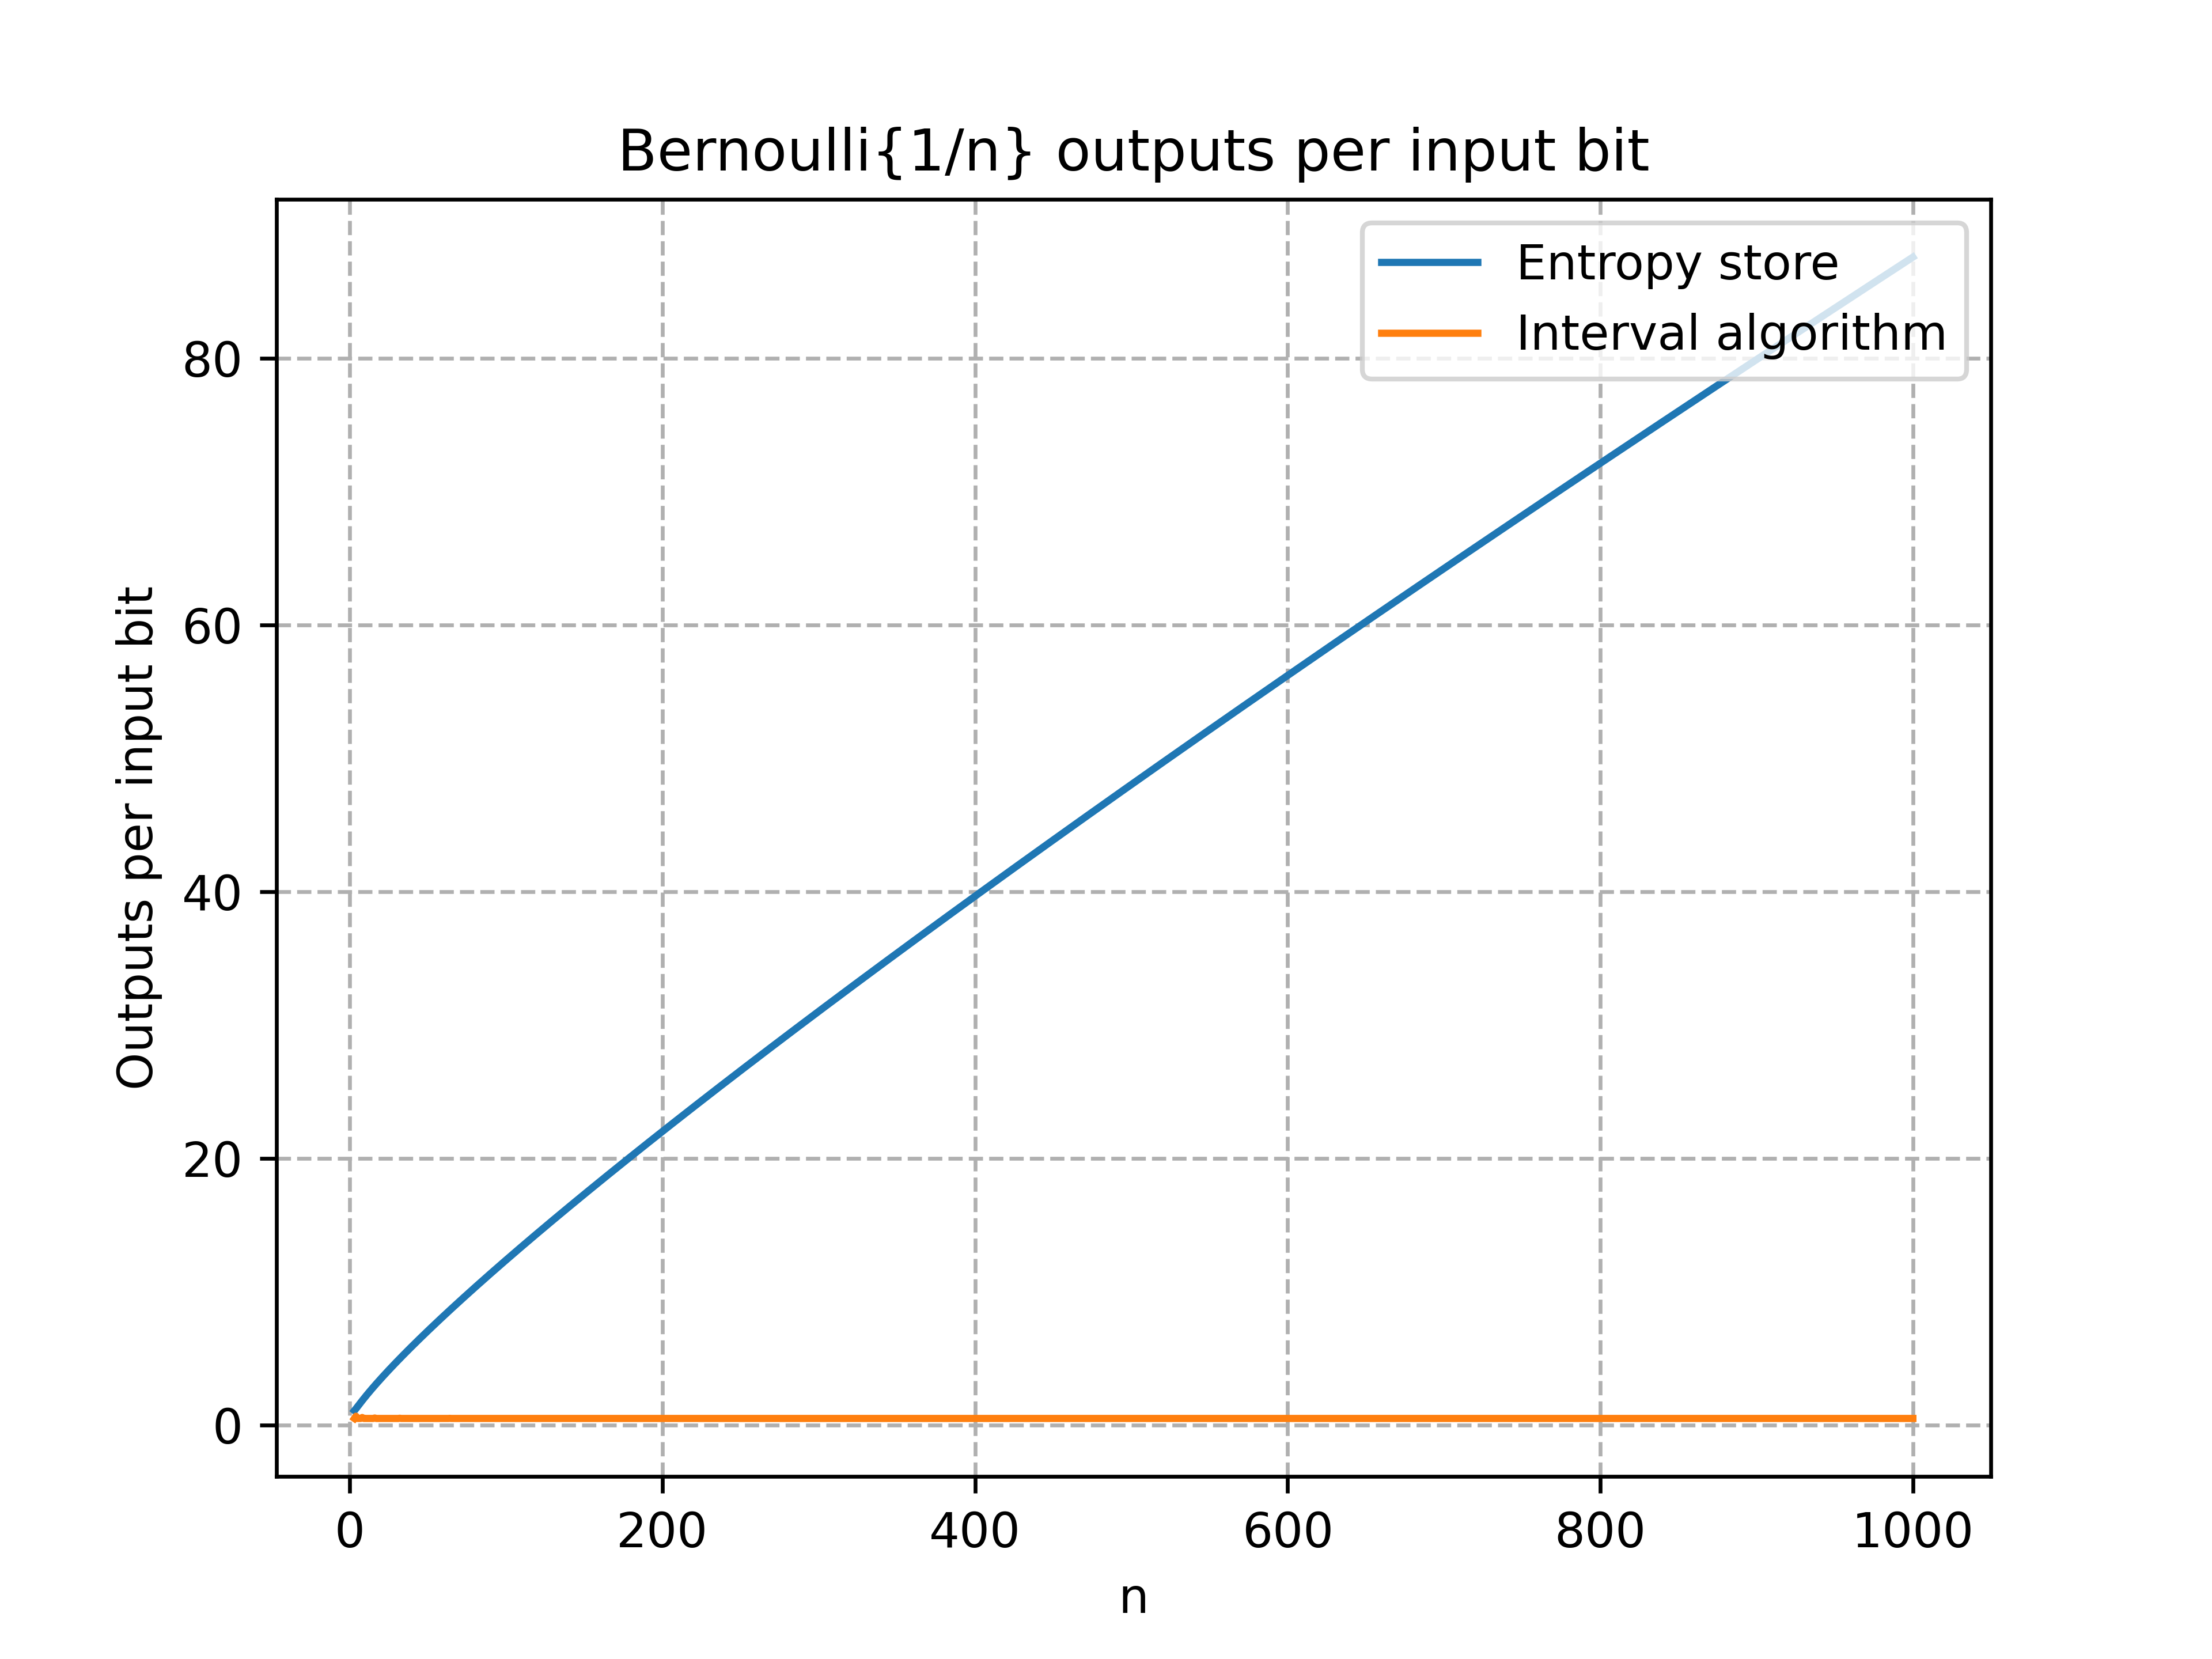
\includegraphics[width=0.8\textwidth]{bernoulli_rate.png}
\caption{Output rate for Bernoulli distributions.}
\label{fig:bernoulli-rate}
\end{figure}

We can also evaluate ES algorithms in terms of memory, speed, setup costs and flexibility. ES can be written to use 2 integer divmod operations (see \ref{appendix}), which are likely to prove a bottleneck compared to say Lemire's algorithm \cite{lemire2019fast}, or table-based algorithms like FLDR \cite{saad2020fldr,saad2025}. Integer division and multiplication is $O(n \log n)$ \cite{harvey2021integer}, for an $m$ bit buffer the complexity of ES is $O(n \log n)$, but for practical purposes it is $O(1)$ in time and space.

ES is able to generate perfect distributions and does not have (albeit minimal) truncation errors found in IA.

The entropy store can be used as part of a Markov sequence for either input or output.

\section{Conclusion}

We have introduced a new class of algorithm to convert entropy via a uniform entropy store efficiently, and by caching unused entropy between outputs we can achieve arbitrarily low entropy losses.

We have shown that the entropy efficiency limits of classical algorithms like Knuth-Yao and the Interval Algorithm can be avoided by using an entropy store. 

The ES algorithms are simple and practical enough to be of use in low entropy regimes where the availability of entropy is a bottleneck. The difference with classical algorithms is particularly marked on Bernoulli outputs.

A drawback with the method is the need for 2 divmod operations per output. It would be very interesting to see if ES methods could found that avoid integer division entirely.






\printbibliography

\section {Appendix A}
Source code for $generate\_uniform$, written in C.

\begin{verbatim}
    const uint32_t N = 1<<31;
    uint32_t s_value = 0, s_range = 1;

    uint32_t generate_uniform(uint32_t n)
    {
        for(;;)
        {
            // Preload entropy one bit at a time into s
            while(s_range < N)
            {
                s_value <<= 1;
                s_value |= fetch();
                s_range <<= 1;
            }
            // Resample entropy s to a multiple of n
            uint32_t r = s_range / n;
            uint32_t c = s_range % n;
            if(s_value >= c)
            {
                // Resample successful
                s_value -= c;
                uint32_t a = s_value / n;
                uint32_t b = s_value % n;
                s_value = a;
                s_range = r; 
                return b;
            }
            else
            {
                // Resample unsuccessful
                s_range = c;
            }
        }
    }
\end{verbatim}

\end{document}
